% geom.tex
\documentclass[tikz,border=1pt]{standalone}
\begin{document}
	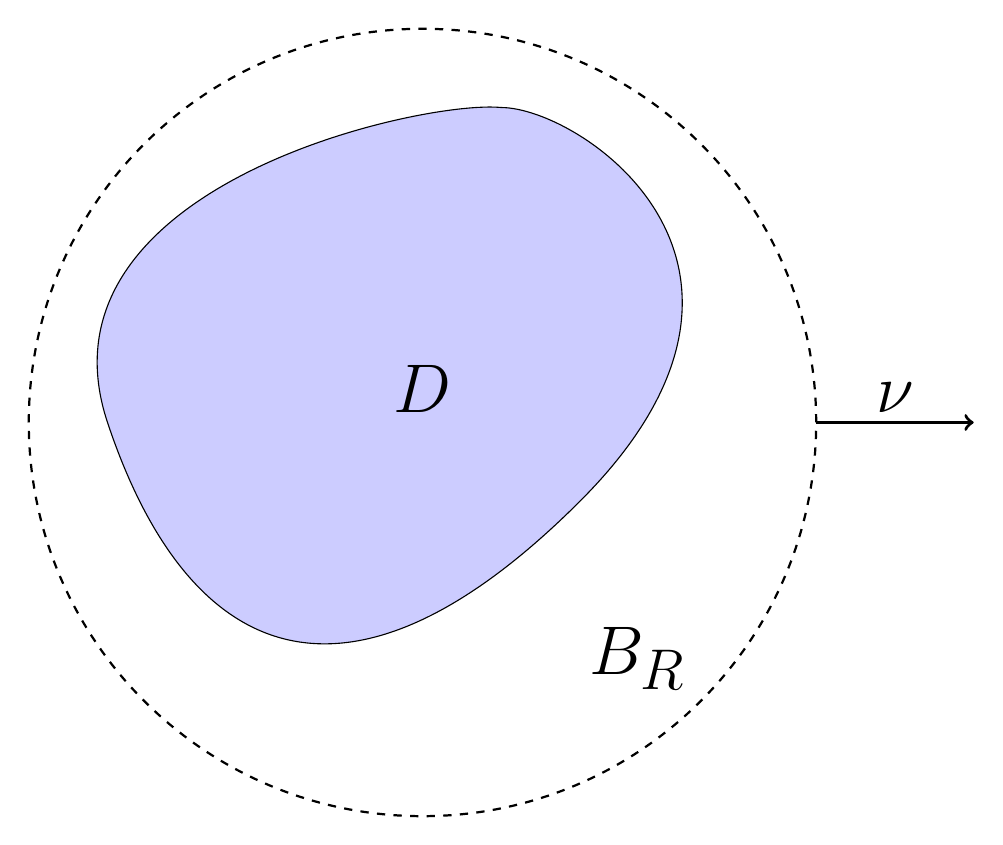
\begin{tikzpicture}
		% artificial boundary
		\draw[dashed,thick] (0, 0) circle [radius=5cm];
		\draw (2, -3) node [right] {\Huge$B_{R}$};
		
		% normal vector
		\draw[->,very thick] (5, 0) -- (7, 0);
		\draw (6, 0) node [above] {\Huge$\nu$};
		
		% domain
		\draw[fill,color=blue!20,draw=black] (-4, 0) .. controls (-3, -3) and (-1, -4) .. 
											 (2, -1) .. controls (5, 2) and (2, 4) .. 
											 (1, 4) .. controls (0, 4.1) and (-5, 3) .. 
											 (-4, 0) -- cycle;
		\draw (0, 0) node [above] {\Huge$D$};
		
	\end{tikzpicture}
\end{document}